\section{Theorie}
\label{Theorie}

Trifft ein Neutron auf ein Atomkern, so erhöht sich dessen Energie um die Bindungsenergie zwischen Neutron und Kern und zusätzlich um die kinetische Energie vom Ersteren. Dadurch können die Energiezustände der Nukleonen im Atomkern verändert werden, weil sie diese Energie in diskreten Massen absorbieren. So kommt folgende Reaktionsgleichung zustande:

%die allererste Reaktionsgleichung auf der Anleitung hier rein
\begin{equation}
    \ce{^{m}_{Z}A}\ +\ \ce{^1_0n}\ \to\ \ce{^{m+1}_{Z}A^{*}}\ \to \ \ce{^{m+1}_{Z}A}\ +\ \gamma
\end{equation}

wobei \(A^{*}\) der Kern im angeregten Zustand ist, \(m\) die Massenzahl, \(z\) die Ordnungszahl, \(n\) das Neutron und \(\gamma\) ein freigesetztes Neutrino ist.\\
Da der Kern mit der erhöhten Massenzahl allerdings nicht stabil ist, emittiert es zusätzlich noch ein Elektron auf Kosten seiner Ordnungszahl, die sich dann um eins erhöht.\\
Die Wahrscheinlichkeit dafür, dass das Einfangen eines Neutrons überhaupt geschieht, heißt Wirkungsquerschnitt \(\sigma\). Diese lässt sich wie folgt berechnen:

\begin{equation}
    \sigma = \frac{u}{nKd}.
\end{equation}

\(u\) ist hierbei die Anzahl der Einfänge, \(n\) die Anzahl der Neutronen, \(d\) die Dicke der Folie, die zum EInfangen der Neutronen benutzt wurde und \(K\) die Anzahl der Atome pro Volumeneinheit.\\
Resonanzabsorption tritt auf, wenn die Energie eines einfallenden Neutrons gleich der Differenz zwischen zwei Energieniveaus des Kern ist, was anhand des Wirkungsquerschnitts und sein Maximum ersichtlich wird. Diese lautet hierbei

\begin{equation}
    \sigma(E) = \sigma_0 \sqrt{\frac{E_{r,i}}{E}} \frac{C}{(E-E_{r,i})^2 + C},
\end{equation}

wobei \(C\) und \(\sigma_0\) charakteristische Konstanten der Kernreaktionen sind.\\
Die Neutronen, die eine niedrige Energie haben, können durch Alphazerfälle erzeugt werden. Bei elastischen Stößen an Kernen wird folgende Energie übertragen:

\begin{equation}
    E_ü = E_0 \frac{4Mm}{(M+m)^2},
\end{equation}

wobei \(m\) und \(M\) die Massen des Neutrons und des Atomkerns sind.\\
Das Zerfallsgesetz lautet hierbei:

\begin{equation}
    N(t) = N_0 e^{-\lambda t}.
\end{equation}

\(N\) ist hier die Anzahl der noch nicht zerfallenen Kerne, \(\lambda\) die Zerfallskonstante und \(t\) die vergangene Zeit. Die Halbwertszeit ist der Zeitpunkt, zu der nur noch die Hälfte der noch nicht zerfallenen Kerne bestehen geblieben sind. Daher lautet \(T_{\frac{1}{2}}\) immer:

\begin{equation}
    T_{\frac{1}{2}} = \frac{\ln{2}}{\lambda}.
    \label{eq:hwz}
\end{equation}

\(N(t)\) erweist sich als schwierig zu messen, weshalb stattdessen die Anzahl der zerfallenen Kerne in einem festen Zeitintervall \(\Delta t\) gemessen und daraus ein \(N_{\Delta t}(t)\) ermittelt wird. Diese ist dann definiert als

\begin{equation}
    N_{\Delta t}(t) = N_0(1-e^{-\lambda \Delta t})e^{-\lambda t}.
\end{equation}

Dabei sollte das Zeitintervall für die Messungen nicht zu klein oder zu groß sein, um gravierende Fehler zu vermeiden. Bei Silber und Rhodium treten allerdings Probleme auf:\\
Das Isotop des Rhodium zerfällt mit unterschiedlichen Wahrscheinlichkeiten in zwei verschiedenen Isotopen. Sie haben auch unterschiedliche Halbwertszeiten. Beide Aktiviäten, welche als Ableitung von \(N(t)\) definiert sind, müssen für die Gesamntaktivität addiert werden.\\
Dasselbe geschieht bei Silber.\\
Die ermittlung der einzelnen Aktivitäten erfolgt mithilfe von Ausgleichsgeraden, deren Zerfallskonstanten unterschiedlich sind:

\begin{figure}
    \centering
    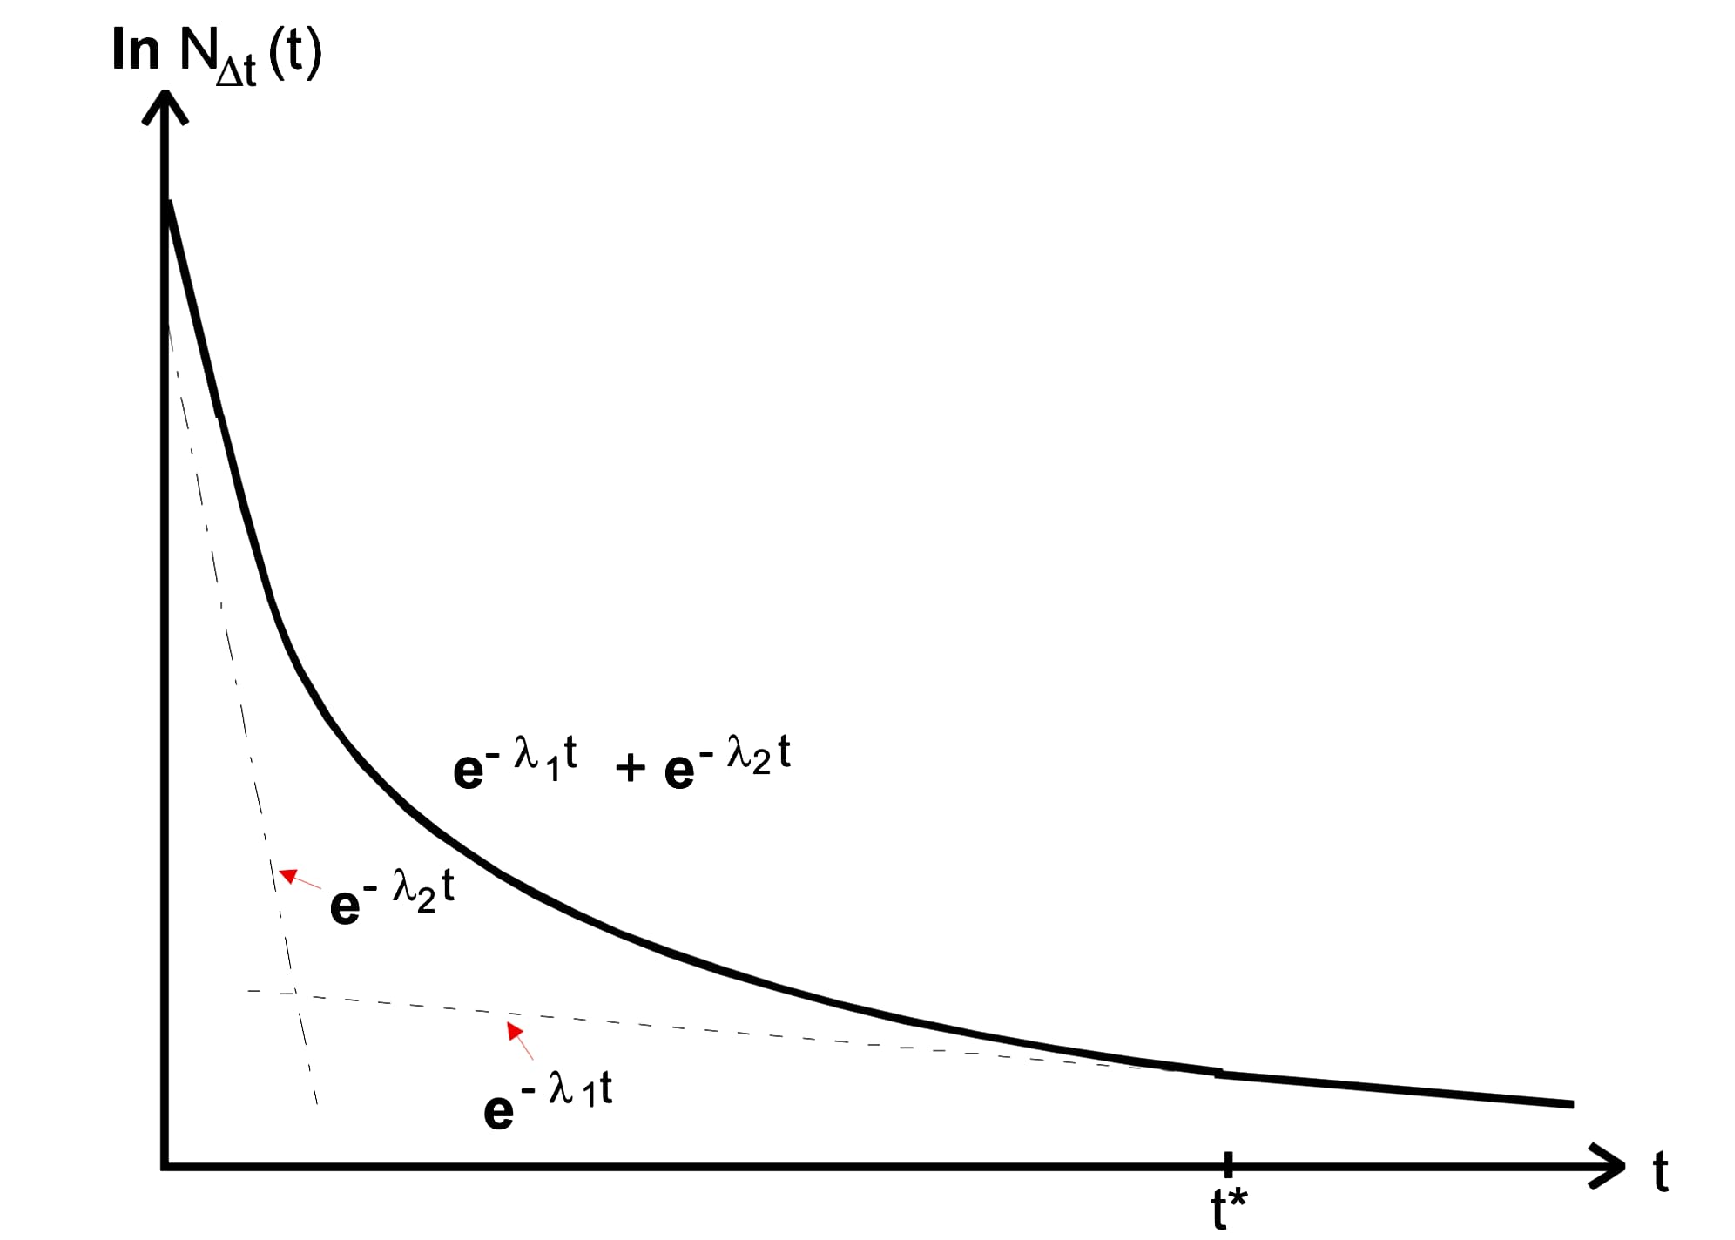
\includegraphics[scale = 0.4]{content/Zerfall.pdf}
    \caption{Hier zu sehen ist eine Skizze, welche das Vorgehen zur Bestimmung beider einzelnen Zerfälle beschreibt. Hierbei ist anzumerken, dass die Differenz der einzelnen Zerfallskonstanten sehr groß sein muss. In diesem Fall gilt \(\lambda_2\) << \(\lambda_1\).}
    \label{fig:zerfall}
\end{figure}


%Theorie klappt (ohne Reaktionsgleichung)!